%%%%%%%%%%%%%%%%%%%% book.tex %%%%%%%%%%%%%%%%%%%%%%%%%%%%%

\documentclass[english, 11pt]{book}

\usepackage{babel}
% choose options for [] as required from the list
% in the Reference Guide, Sect. 2.2

\usepackage{makeidx}         % allows index generation
\usepackage{graphicx}        % standard LaTeX graphics tool
                             % when including figure files
\usepackage{multicol}        % used for the two-column index
\usepackage[bottom]{footmisc}% places footnotes at page bottom
% etc.
% see the list of further useful packages
% in the Reference Guide, Sects. 2.3, 3.1-3.3
\usepackage[normalem]{ulem}

\usepackage[shortlabels]{enumitem}	% to be able to resume enumerated lists

\usepackage{amsmath}	% To be able to slash
\usepackage{amsfonts}	% To be able to use \mathbb ... 
\usepackage{amssymb}	% To be able to use \nmid ... 
\usepackage{amsthm}		% \qed, \qedhere
\usepackage{slashed}	% any character (dirac)
% Physics package 
% https://tex.stackexchange.com/questions/38978/how-can-i-manually-install-a-latex-package-debian-ubuntu-linux
\usepackage{physics}	
\usepackage[title,toc,page]{appendix}

% To put accents below letters
\usepackage{accents}
% To write two equations side by side
\usepackage{multicol}

% To use PGF/TikZ https://tex.stackexchange.com/questions/3622/best-way-to-generate-nice-function-plots-in-latex
\usepackage{tikz}
\usetikzlibrary{datavisualization}
\usetikzlibrary{datavisualization.formats.functions}

% Force chapter numbering to restart within each part
\makeatletter
%\@addtoreset{chapter}{part}
\makeatletter


\makeindex             % used for the subject index
                       % please use the style svind.ist with
                       % your makeindex program


%%%%%%%%%%%%%%%%%%%%%%%%%%%%%%%%%%%%%%%%%%%%%%%%%%%%%%%%%%%%%%%%%%%%%

\begin{document}

\newcommand{\quotes}[1]{``#1''}
\newcommand{\sfT}{$\mathsf{T}$}
\newcommand{\udT}{\rotatebox[origin=c]{180}{$\mathsf{T}$}}
\newcommand{\N}{\mathbb{N}}
\newcommand{\Z}{\mathbb{Z}}
\newcommand{\Q}{\mathbb{Q}}
\newcommand{\R}{\mathbb{R}}
\newcommand{\C}{\mathbb{C}}

% To put accents below letters. Here \form{\theta} put a tilde below 
\newcommand{\ut}[1]{\underaccent{\tilde}{#1}}
\newcommand{\uh}[1]{\underaccent{\hat}{#1}}
\newcommand{\form}[1]{\uh{#1}}

% To create italic, bold, bolditalic text
\newcommand{\tit}[1]{\textit{#1}}
\newcommand{\tbf}[1]{\textbf{#1}}
\newcommand{\tbi}[1]{\textit{\textbf{#1}}}


\DeclareRobustCommand{\rchi}{{\mathpalette\irchi\relax}}
\newcommand{\irchi}[2]{\raisebox{\depth}{$#1\chi$}} % inner command, used by \rchi

%----------------------------------------------------------------------------------------
%   r Griffiths, curls and fonts from mt2pro[lite]->pro
%----------------------------------------------------------------------------------------
%\def\rcurs{s}
%\def\brcurs{\vb{\rcurs}}
%\def\hrcurs{\vu{\rcurs}}


\author{Marcello Vitaletti}
\title{Notes on the Classical Theory of Fields\\
{\small }}
\maketitle

\frontmatter%%%%%%%%%%%%%%%%%%%%%%%%%%%%%%%%%%%%%%%%%%%%%%%%%%%%%%

%\include{dedic}

%\chapter*{Plan}
\label{plan} 

In this book I am keeping notes about the theory of classical electromagnetism, 
as exposed in various books. In particular, I intend to cover the following materials:

\begin{itemize}

\item B. Felsager -- Geometry Particles and Fields
\begin{enumerate}
\setcounter{enumi}{0}
\item Electromagnetism (1.1 to 1.4)
\end{enumerate}

\item C. Cattaneo -- Teoria Einsteniana della Gravitazione
\begin{enumerate}
\setcounter{enumi}{0}
\item Elementi di Algebra e Analisi Lineare
\end{enumerate}

\item D.J. Griffiths -- Introduction to Electrodynamics
\begin{enumerate}
\setcounter{enumi}{0}
\item Vector Analysis
\item Electrostatics
\item Potentials
\item Electric Fields in Matter
\item Magnetostatics
\item Magnetic Fields in Matter
\item Electrodynamics
\item Conservation Laws
\item Electromagnetic Waves
\item Radiation
\item Electrodynamics and Relativity
\item Potentials and Fields
\item Helmoltz Theorem
\end{enumerate}

\item J.D. Jackson -- Classical Electrodynamics, 2nd Edition
\begin{enumerate}
\setcounter{enumi}{0}
\item Introduction to Electrostatics
\item Boundary Value Problems in Electrostatics - I
\item Boundary Value Problems in Electrostatics - II
\item Multipoles, Electrostatics of Macroscopic Media, Dielectrics
%\item Magnetostatics
%\item Time Varying Fields, Maxwell Equations, Conservation Laws
%\item Plane Electromagnetic Waves and Wave Propagation
%\item Wave Guides and Resonant Cavities
%\item Simple Radiating Systems, Scattering and Diffraction
%\item Magnetohydrodynamics and Plasma Physics
\end{enumerate}

\item J.D. Jackson -- Classical Electrodynamics, 3rd Edition
\begin{enumerate}
\setcounter{enumi}{4}
\item Magnetostatics, Faraday's Law, Quasi-Static Fields
\item Maxwell Equations, Macroscopic Electromagnetism, Conservation Laws
\item Plane Electromagnetic Waves and Wave Propagation
\item Wave Guides, Resonant Cavities and Optical Fibers
\item Radiating Systems, Multipole Fields and Radiation
\item Scattering and Diffraction
\item Special Theory of Relativity
\item Dynamics of Relativistic Particles and Electromagnetic Fields
\end{enumerate}

\item B. Felsager -- Geometry Particles and Fields
% Contacts with quantum theory of particles dynamics in EM fields
\begin{enumerate}
\setcounter{enumi}{1}
\item Interaction of Fields and Particles
\end{enumerate}

\item J. Franklin -- Advanced Mechanics and General Relativity
\begin{enumerate}
\setcounter{enumi}{1}
\item Relativistic Mechanics
\item Tensors
\item Curved Space
\item Scalar Field Theory
\item Tensor Field Theory (6.1 to 6.5)
\end{enumerate}

\item J.D. Jackson -- Classical Electrodynamics, 3rd Edition
\begin{enumerate}
\setcounter{enumi}{12}
\item Collisions, Energy Loss and Scattering of Charged Particles, Cherenkov and Transition Radiation
\item Radiation by Moving Charges
\item Bremsstrahlung, Method of Virtual Quanta, Radiative Beta Processes
\item Radiation Damping, Classical Models of Charged Particles
\end{enumerate}

\item B. Felsager -- Geometry Particles and Fields
% Contacts with quantum theory of fields dynamics + differential geometry math
\begin{enumerate}
\setcounter{enumi}{2}
\item Dynamics of Classical Fields
\end{enumerate}

\begin{enumerate}
\setcounter{enumi}{5}
\item Differentiable Manifolds, Tensor analysis
\item Differential Forms, Exterior Calculus
\item Integral Calculus on Manifolds
\end{enumerate}

\item C.W. Misner, K.S. Thorne, J.A. Wheeler -- Gravitation
\begin{enumerate}
\setcounter{enumi}{1}
\item Foundations of Special Relativity
\item The Electromagnetic Field
\item Electromagnetism and Differential Forms
\end{enumerate}

\item L.D. Landau, E.M. Lifshitz -- Teoria dei Campi
\begin{enumerate}
\setcounter{enumi}{0}
\item Principio di Relatività
\item Meccanica Relativistica
\item Carica in un Campo Elettromagnetico
\item Equazioni del Campo Elettromagnetico
\item Campo Elettromagnetico Costante
\item Onde Elettromagnetiche
\item Propagazione della Luce
\item Campo di Cariche in Moto
\item Radiazione Elettromagnetica
\end{enumerate}

\item L.D. Landau, E.M. Lifshitz -- Elettrodinamica dei Mezzi Continui
\begin{enumerate}
\setcounter{enumi}{0}
\item Elettrostatica dei Conduttori
\item Elettrostatica nei Dielettrici
\item Corrente Continua
\item Campo Magnetico Costante
\item Ferromgnetismo e Antiferromagnetismo
\item Superconduttività
\item Campo Magnetico Quasi Stazionario
\item Idrodinamica Magnetica
\item Equazioni delle Onde Elettromagnetiche
\item Propagazione delle Onde Elettromagnetiche
\item Onde Elettromagnetiche in Mezzi Anisotropi
\item Dispersione Spaziale
\item Ottica non Lineare
\item Passaggio delle Particelle Veloci attraverso la Materia
\item Diffusione delle Onde Elettromagnetiche
\item Diffrazione dei Raggi X nei Cristalli
\end{enumerate}

\end{itemize}
	
\tableofcontents
%\addappheadtotoc

\mainmatter%%%%%%%%%%%%%%%%%%%%%%%%%%%%%%%%%%%%%%%%%%%%%%%%%%%%%%%

\chapter{Franklin -- Newton Gravity}
\label{ch:Franklin_01} 

   % Franklin  - Advanced Mechanics and General Relativity - Newton Gravity
%\chapter{Felsager -- Electromagnetism}
\label{felsager_01} 

\section{The Electromagnetic Field}

The two fundamental quantities of the electromagnetic field are the field strenghts

\begin{equation*}
\vb{E}(\vb{r}, t); \:\:\: \vb{B}(\vb{r}, t)
\end{equation*}

$\vb{E}$ is an ordinary (i.e. \textit{polar}) vector field, and as such it can be defined before any choice of a reference system. Instead, $\vb{B}$ is an \textit{axial} vector field and thus it can only be specified with respect to a given reference system. Reference systems can be separated in two \textit{equivalence} classes (a.k.a \textit{orientations}), according to the sign (positive or negative) of the determinant associated to the transformation between two such systems. 

Both polar and axial vectors transform in the same way under spatial \textit{rotations} (a rotation connects two systems with the same orientation). Different behaviors arise when dealing with a \textit{reflection} of the three coordinate axes. This one connects two systems with opposite orientations. Polar vectors are not affected at all by this transformation while any axial vector turns into its opposite.

A large set of experimental data can be interpreted as the manifestation of the \textit{Lorentz} force, defining the effects of the fields $\vb{E}$ and $\vb{B}$ on a particle possessing a \textit{charge} $q$

\begin{equation}
\vb{F}(\vb{r}, t) = q \left(\vb{E}(\vb{r}, t) + \frac{1}{c} \vb{v} \cross \vb{B}(\vb{r}, t) \right)
\label{eq:Lorentzforce1}
\end{equation}

It should be noted that $\vb{v} \cross \vb{B}$ is an ordinary (\textit{polar}) vector because $\vb{B}$ is an axial vector and $\vb{v}$ is an ordinary vector. 

According to special relativity the particle's motion obeys the following equations 

\begin{equation}
\dv{\vb{p}}{t} = q \left(\vb{E} + \frac{1}{c} \vb{v} \cross \vb{B} \right) ; \:\: \vb{p} = \gamma m \vb{v} ; \:\: \gamma = \frac{1}{\sqrt{1 - \frac{v^2}{c^2}}}
\label{eq:Lorentzforce2}
\end{equation}

This relation is of extreme importance and it actually serves to define the electromagnetic field. The argument is that the charge being small allows one to neglect the influence of the particle on the electromagnetic field\footnote{The field generated by the charge is certainly very large in its proximity, so for the argument to work one must assume a charge not to be subject to its own field.}, so that by analyzing the motion of a swarm of particles through the electromagnetic field one can determine the field strenghts $\vb{E}$ and $\vb{B}$.

In 1860 Maxwell derived the equations governing the motion of the electromagnetic field:

\begin{subequations}
\label{eq:Maxwell}
\begin{align}
\div{\vb{B}} &= 0 \label{eq:maxwell_divB}\\
\curl{\vb{E}} + \frac{1}{c} \pdv{\vb{B}}{t} &= 0 \label{eq:maxwell_rotE}\\
\div{\vb{E}} &= 4 \pi \rho \label{eq:maxwell_divE}\\
\curl{\vb{B}} &= \frac{4 \pi}{c} \vb{J} + \frac{1}{c} \pdv{\vb{E}}{t} \label{eq:maxwell_rotB}
\end{align}
\end{subequations}

where $\rho = \rho(\vb{r}, t)$ is the \textit{charge}  density, $\vb{J} = \rho \vb{v}$  the \textit{current}  and $c$ a constant equal to the speed of light in empty space. 

\subsection*{Vector calculus}
%Some formulas of vector calculus are reproduced here to help in the following sections
 
\begin{subequations}
\label{eq:vcalc}
\begin{align}
\vb{A} \cross \vb{B} &= - \vb{B} \cross \vb{A} \label{eq:vcalc_a}\\
\vb{A} \vdot (\vb{B} \cross \vb{C}) &= (\vb{A} \cross \vb{B}) \vdot \vb{C}) \label{eq:vcalc_b}\\
\vb{A} \cross (\vb{B} \cross \vb{C}) &= \vb{B} (\vb{A} \vdot \vb{C}) - (\vb{A} \vdot \vb{B})\vb{C} \label{eq:vcalc_c}\\
(\vb{A} \cross \vb{B}) \cross \vb{C} &= (\vb{A} \vdot \vb{C}) \vb{B} - \vb{A} (\vb{B} \vdot \vb{C}) \label{eq:vcalc_d}\\
\div{(\grad{\phi})} &= \laplacian{\phi} \label{eq:vcalc_e}\\
\curl{(\grad{\phi})} &= \vb{0} \label{eq:vcalc_f}\\
\div{(\curl{\vb{B}})} &= 0 \label{eq:vcalc_g}\\
\curl{(\curl{\vb{B}})} &= \grad(\div{\vb{B}}) - \laplacian{\vb{B}}  \label{eq:vcalc_h}
\end{align}
\end{subequations}

\textbf{Gauss' theorem}

\begin{equation}
\int\limits_{\Omega}\div{\vb{E}} \; \mathrm{d}V = \int\limits_{S}\vb{E} \vdot \vu{n} \; \mathrm{d}A \label{eq:Gauss}
\end{equation}

\textbf{Stokes' theorem}

\begin{equation}
\int\limits_{S}(\curl{\vb{B}}) \vdot \vu{n} \; \mathrm{d}A = \oint\limits_{\Gamma} \vb{B} \vdot \mathrm{d}\vb{r}  \label{eq:Stokes}
\end{equation}

\textbf{Theorem of line-integrals}\\
The integral of the gradient of a scalar function $\phi$ between points $P$ and $Q$ along a curve $\Gamma$ is
  
\begin{equation*}
\int\limits_{\Gamma} \grad{\phi} \vdot \mathrm{d}\vb{r} = \phi(Q) - \phi(P)  \label{eq:LineInt}
\end{equation*}


\subsection*{Charge conservation}
By taking the divergence of \ref{eq:maxwell_rotB} and considering calculus rule \ref{eq:vcalc_g}

\begin{align*}
0 &= \div{(\curl{\vb{B}})} = \frac{4 \pi}{c} \div{\vb{J}} + \frac{1}{c} \pdv{\div{\vb{E}}}{t}
\end{align*}

In force of equation \ref{eq:maxwell_divE} the divergence appearing in the last term can be replaced by $4\pi\rho$ yelding the so called \textit{equation of continuity}  

\begin{equation}
\pdv{\rho}{t} + \div{\vb{J}}= 0 \label{eq:continuity}
\end{equation}

The physical significance of the above equation becomes more evident by applying Gauss' theorem to a control volume $\Omega$ to determine the rate of change of the total charge $Q$ contained inside that volume. Indeed, by definition the total charge located within the control volume at a given point in time is

\begin{equation*}
Q(t) = \int\limits_{\Omega}\rho(t) \; \mathrm{d}V 
\end{equation*}

while the istantaneous \textit{flux} of charge (charge entering or leaving the control volume in a unit of time) is given by the surface integral

\begin{equation*}
\int\limits_{S}\rho \,\vb{v} \vdot \vu{n} \; \mathrm{d}A = \int\limits_{S} \vb{J} \vdot \vu{n} \; \mathrm{d}A 
\end{equation*}

The continuity equation \ref{eq:continuity} just links, via the Gauss' theorem, the total flux of charge to the rate of change of $Q$  

\begin{equation*}
\frac{\mathrm{d} \, Q(t)}{\mathrm{d} \, t}  = \int\limits_{\Omega} \pdv{\rho}{t} \; \mathrm{d}V = - \int\limits_{S}\vb{J} \vdot \vu{n} \; \mathrm{d}A 
\end{equation*}

This result is equivalent to the assertion that a decrease[increase] of the total charge in the control volume $V$ by an amount $\mathrm{d}Q$ does always occur if and only if an equal amount of charge flows across the boundary toward the exterior[interior] of the control volume during the same amount of time. 

In short, electric charge is not created nor destroyed by electromagnetic processes. 

\section{Gauge Potentials in Electromagnetism}

Identities \ref{eq:vcalc_f} and \ref{eq:vcalc_g} from vector calculus can be exploited to express the fields $\vb{E}$ and $\vb{B}$ in terms of a \textit{scalar} field $\phi$ and a \textit{vector} field $\vb{A}$, thus causing the \textit{homogeneous} Maxwell equations \ref{eq:maxwell_divB} and \ref{eq:maxwell_rotE} to be automatically satisfied. 

Indeed, by equating $\vb{B}$ to the curl of a \textit{vector} field $\vb{A}$ the divergence of $\vb{B}$ does necessarily vanish, as required by \ref{eq:maxwell_divB}:

\begin{equation}
\vb{B} = \curl{\vb{A}} \:\: \longrightarrow \:\: \div{\vb{B}} = \div{(\curl{\vb{A}})} = 0 \label{eq:Bdef}
\end{equation}
   
Once $\vb{B}$ satisfies \ref{eq:Bdef}, the companion Maxwell equation \ref{eq:maxwell_rotE} reads:

\begin{equation*}
\curl{\vb{E}} + \frac{1}{c} \pdv{\vb{B}}{t} = \curl{\left( \vb{E} + \frac{1}{c} \pdv{\vb{A}}{t} \right)} = 0 
\end{equation*}
 
Therefore, by equating the argument of the curl operator in the above equation to the \textit{gradient} of a \textit{scalar} field $\phi$ the Maxwell equation  \ref{eq:maxwell_rotE} is automatically satisfied:

\begin{equation}
\left( \vb{E} + \frac{1}{c} \pdv{\vb{A}}{t} \right) = - \grad{\phi} \:\: \longrightarrow \:\: \curl{\vb{E}} + \frac{1}{c} \pdv{\vb{B}}{t} = - \curl{(\grad{\phi})} = \vb{0} \label{eq:Edef}
\end{equation}

What we have demonstrated so far is that the fields can be conveniently expressed in terms of the potentials $\phi$ and $\vb{A}$ as follows

\begin{subequations}
\label{eq:potentials_1}
\begin{align}
\vb{B} &= \curl{\vb{A}} \label{eq:potentials_11} \\
\vb{E} &= - \grad{\phi} - \frac{1}{c} \pdv{\vb{A}}{t} \label{eq:potentials_12} 
\end{align}
\end{subequations}

It is important to note that the equations \ref{eq:potentials_1} do not restrict the range of admissible solutions to the Maxwell equations \ref{eq:Maxwell}\footnote{We are aassuming, without demonstration, that any vector field with zero divergence is the curl of some vector potential and one with zero curl is the gradient of some scalar potential.}. 

By substituting the equations \ref{eq:potentials_1} in the two \textit{inhomogeneous} Maxwell equations \ref{eq:maxwell_divE} and \ref{eq:maxwell_rotB} we get the potential dependency from \textit{sources}: 

\begin{align*}
- \div{\vb{E}} &= - 4 \pi \rho \\
			&= \laplacian{\phi} + \frac{1}{c} \pdv{\div{\vb{A}}}{t} \\
- \curl{\vb{B}} &= - \curl{(\curl{\vb{A}})} \\
			&= \laplacian{\vb{A}} - \grad{(\div{\vb{A})}} \\
			&= - \frac{4 \pi}{c} \vb{J} - \frac{1}{c} \pdv{\vb{E}}{t} \\
			&= - \frac{4 \pi}{c} \vb{J} + \frac{1}{c} \pdv{}{t} \left( \grad{\phi} + \frac{1}{c} \pdv{\vb{A}}{t}   \right)	
\end{align*}

Terms in the above equations can be rearranged to give 
\begin{align*}
\Box \, \phi &= \laplacian{\phi} - \frac{1}{c^2} \pdv[2]{\phi}{t} \\
			&= - 4 \pi \rho - \frac{1}{c} \pdv{\div{\vb{A}}}{t} - \frac{1}{c^2} \pdv[2]{\phi}{t} \\
			&= - 4 \pi \rho - \frac{1}{c} \pdv{}{t} \left( \div{\vb{A}} + \frac{1}{c} \pdv{\phi}{t}  \right) \\
\Box \, \vb{A} &= \laplacian{\vb{A}} - \frac{1}{c^2} \pdv[2]{\vb{A}}{t} \\
			&= - \frac{4 \pi}{c} \vb{J} + \frac{1}{c} \pdv{}{t} \left( \grad{\phi} + \frac{1}{c} \pdv{\vb{A}}{t}   \right) + \grad{(\div{\vb{A})}} - \frac{1}{c^2} \pdv[2]{\vb{A}}{t} \\
			&= - \frac{4 \pi}{c} \vb{J} + \frac{1}{c} \pdv{}{t} \left( \grad{\phi} \right) + \grad{(\div{\vb{A})}} \\
			&= - \frac{4 \pi}{c} \vb{J} + \grad{\left( \div{\vb{A}} + \frac{1}{c} \pdv{\phi}{t}  \right)}
\end{align*}

The above tour de force is summarized in the following two equations:
 
\begin{subequations}
\label{eq:potentials_2}
\begin{align} 
\Box \, \phi &= - 4 \pi \rho - \frac{1}{c} \pdv{}{t} \left( \div{\vb{A}} + \frac{1}{c} \pdv{\phi}{t}  \right)
\label{eq:potentials_21} \\
\Box \, \vb{A} &= - \frac{4 \pi}{c} \vb{J} + \grad{\left( \div{\vb{A}} + \frac{1}{c} \pdv{\phi}{t}  \right)}
\label{eq:potentials_22} 
\end{align}
\end{subequations}

The term appearing between parentheses causes an unwanted coupling of the two equations. Fortunately, we have still freedom left in the choice of potentials to get rid of this term. Indeed...


 
   % Felsager  - Electromagnetism

\chapter{Griffiths -- Vector Analysis}
\label{Griffiths_00} 

\section{Vector Algebra}
For the sake of fixing notation, let $\{\vu{i}, \vu{j}, \vu{k}\}$ be an \textit{orthonormal} basis of unit vectors in three-dimensional space, and the following a list of all possible scalar products of basis vectors. 
  
\begin{equation}
\begin{aligned} 
\vu{i}\vdot \vu{i} &= \vu{j} \vdot \vu{j} = \vu{k} \vdot \vu{k} = 1 \\ 
\vu{i} \vdot \vu{j} &= \vu{j} \vdot \vu{k} = \vu{k} \vdot \vu{i} = 0 
\label{eq:basis_dot_products}
\end{aligned}
\end{equation}

For a \textit{right-handed} basis, the following is a list of all possible \textit{vector} products of basis vectors.
  
\begin{equation}
\begin{aligned} 
\vu{i} \cross \vu{i} &= \vu{j} \cross \vu{j} = \vu{k} \cross \vu{k} = 0 \\ 
\vu{i} \cross \vu{j} &= \vu{k} = - \vu{j} \cross \vu{i}\\
\vu{j} \cross \vu{k} &= \vu{i} = - \vu{k} \cross \vu{j}\\
\vu{k} \cross \vu{i} &= \vu{j} = - \vu{i} \cross \vu{k}
\label{eq:basis_vector_products}
\end{aligned}
\end{equation}

Any vector $\vb{A}$ can be resolved into a linear combination of the basis vectors
\begin{equation*}
\vb{A} = A_x \, \vu{i} + A_y \, \vu{j} + A_z \, \vu{k} 
\end{equation*}

where $A_x, A_y, A_z$ are the vector \textit{components} in that basis. 

When the basis is assumed, a list of comma separated numbers within parentheses indicate the components of a vector in that basis: 

\begin{equation*}
(A_x, A_y, A_z) \equiv \vb{A} = A_x  \vu{i} + A_y  \vu{j} + A_z  \vu{k} 
\end{equation*}

The \textit{dot} product of two vectors is the \textit{scalar}  
\begin{equation}
\vb{A} \vdot \vb{B} = A_x B_x + A_y B_y + A_z B_z 
\label{eq:dot_product}
\end{equation}

The \textit{cross} product of two vectors is the \textit{vector}  
\begin{equation}
\begin{aligned}
\vb{A} \cross \vb{B} &= (A_y B_z - A_z B_y)\, \vu{i} \\
                     &+ (A_z B_x - A_x B_z)\, \vu{j} \\
                     &+ (A_x B_y - A_y B_x)\, \vu{k}
\end{aligned}
\label{eq:cross_product}
\end{equation}

A useful mnemonic expression equivalent to \ref{eq:cross_product} is the \textit{determinant} 
\begin{equation*}
\mqty| \vu{i} &  \vu{j} &  \vu{k} \\ 
A_x & A_y & A_z \\
B_x & B_y & B_z|
\end{equation*}


It follows from \ref{eq:basis_vector_products} that for any two vectors $\vb{A}$ and $\vb{B}$ 
\begin{equation}
\vb{A} \cross \vb{B} = - \vb{B} \cross \vb{A}
\label{eq:cross_product_reflection}
\end{equation}

\subsection{Triple products}
Since the cross product of two vector is itself a vector, it can be dotted or crossed with a third vector to form a \textit{triple} product. 

\subsubsection{Scalar triple product}
The norm of $\vb{A} \vdot (\vb{B} \cross \vb{C})$ is the volume of a parallelepiped generated by $\vb{A}$, $\vb{B}$ and $\vb{C}$, since $\abs{ \vb{B} \cross \vb{C} }$ is the area of the base, while the dot product multiplies that number by the length of the projection of $\vb{A}$ orthogonal to the area. The choice of which vectors make the base of the parallelepiped is arbitrary, while the volume is independent of that choice, therefore: 

\begin{equation}
\vb{A} \vdot (\vb{B} \cross \vb{C}) = \vb{B} \vdot (\vb{C} \cross \vb{A}) = \vb{C} \vdot (\vb{A} \cross \vb{B})
\label{eq:scalar_triple_product}
\end{equation}

When $\vb{A}$, $\vb{B}$ and $\vb{C}$ form a \textit{right-handed} [\textit{left-handed}] basis --not necessarily orthonormal-- the above forms evaluate to the same \textit{positive} [\textit{negative}] value.  

Because of \ref{eq:cross_product_reflection} the following three extra forms are also equivalent among each other but they evaluate to the \textit{opposite} value, thus yielding a \textit{negative} [\textit{positive}] value when $\vb{A}$, $\vb{B}$ and $\vb{C}$ form a \textit{right-handed} [\textit{left-handed}] basis.

\begin{equation}
\vb{A} \vdot (\vb{C} \cross \vb{B}) = \vb{B} \vdot (\vb{A} \cross \vb{C}) = \vb{C} \vdot (\vb{B} \cross \vb{A})
\end{equation}

\subsubsection{Vector triple product}

The vector triple product can be simplified by the $\vb{BAC}\mathbf{-}\vb{CAB}$ rule:
\begin{equation}
\vb{A} \cross (\vb{B} \cross \vb{C}) = \vb{B} (\vb{A} \vdot \vb{C}) - \vb{C} (\vb{A} \vdot \vb{B})
\label{eq:vector_triple_product}
\end{equation}

Note that 

\begin{equation*}
(\vb{A} \cross \vb{B}) \cross \vb{C} = - \vb{C} \cross (\vb{A} \cross \vb{B}) = \vb{B} (\vb{A} \vdot \vb{C}) - \vb{A} (\vb{B} \vdot \vb{C})
\end{equation*}

so changing the grouping yields a different vector, namely

\begin{equation*}
\vb{A} \cross (\vb{B} \cross \vb{C}) - (\vb{A} \cross \vb{B}) \cross \vb{C} = \vb{A} (\vb{B} \vdot \vb{C})  - \vb{C} (\vb{A} \vdot \vb{B})
\end{equation*}

All \textit{higher} products can be similarly reduced, so that it is never necessary for an expression to contain more than one cross product in any term. For instance
\begin{equation}
\begin{aligned} 
(\vb{A} \cross \vb{B}) \vdot (\vb{C} \cross \vb{D}) &= (\vb{A} \vdot \vb{C}) (\vb{B} \vdot \vb{D}) - (\vb{A} \vdot \vb{D}) (\vb{B} \vdot \vb{C})\, ;  \\
\vb{A} \cross [\vb{B} \cross (\vb{C} \cross \vb{D})] &= \vb{B} [\vb{A} \vdot (\vb{C} \cross \vb{D})] -  (\vb{A} \vdot \vb{B})(\vb{C} \cross \vb{D})
\end{aligned}
\end{equation}

\subsubsection{Problem 1}
Prove that 
\begin{equation*}
[\vb{A} \cross (\vb{B} \cross \vb{C})] + [\vb{B} \cross (\vb{C} \cross \vb{A})] +  [\vb{C} \cross (\vb{A} \cross \vb{B})] = 0  
\end{equation*}

By applying the BAC-CAB rule to each one of the above three terms one obtains the following six   terms\footnote{Each line is obtained by the previous one by putting in each place the vector which follows -- in the $ABC$ cycle-- the one in the same place in the line above.}
\begin{equation*}
\begin{aligned} 
\vb{A} (\vb{B} \vdot \vb{C}) &- \vb{C} (\vb{A} \vdot \vb{B})\, +\\
\vb{B} (\vb{C} \vdot \vb{A}) &- \vb{A} (\vb{B} \vdot \vb{C})\, +\\
\vb{C} (\vb{A} \vdot \vb{B}) &- \vb{B} (\vb{C} \vdot \vb{A})
\end{aligned}
\end{equation*}
Each scalar product appears twice, each time it is multiplied by the remaining vector but with opposite signs.\qed. 


\section{Position, Displacement, Separation Vectors}

The vector connecting the origin $\mathcal{O}$ to the location of a point in three dimensions is called the \textbf{position vector}
\begin{equation}
\vb{r} \equiv x \, \vu{i} + y \, \vu{j} + z \, \vu{k} 
\end{equation}

Following Griffiths, we reserve the letter $\vb{r}$ for that purpose. Its magnitude 

\begin{equation}
r = \sqrt{x^2 + y^2 + z^2} 
\end{equation}

is the distance from the origin, and 

\begin{equation}
\vu{r} = \frac{\vb{r}}{r} = \frac{x \, \vu{i} + y \, \vu{j} + z \, \vu{k}}{\sqrt{x^2 + y^2 + z^2}} 
\end{equation}

is a unit vector pointing radially outward. Following Griffiths, the \textbf{infinitesimal displacement vector} from $(x, y, z)$ to $(x+dx, y+dy, z+dz)$ is denoted as $d\vb{l}$

\begin{equation}
d\vb{l} = dx \, \vu{i} + dy \, \vu{j} + dz \, \vu{k} 
\end{equation}

Problems in electrodynamics frequently involve two points, typically a \textbf{source point}, $\vb{r}'$ and a \textbf{field point} $\vb{r}$ at which one needs to calculate the effect of the source. Following Griffiths we reserve the special symbol $\brcurs$ to denote the \textbf{separation vector} from the source point to the field point:

\begin{equation}
\begin{aligned}
\brcurs &\equiv \vb{r} - {\vb{r}}'\\
\rcurs &= \abs{\brcurs} = \abs{\vb{r} - {\vb{r}}'} \\
\hrcurs &= \frac{\brcurs}{\rcurs}
\end{aligned}
\end{equation}


\section{How Vectors Transform}
 




  % Griffiths - Electrodynamics / Vector Analysis
\chapter{Griffiths -- Electrostatics}
\label{ch:Griffiths_01} 

\section{THE ELECTRIC FIELD}
\subsection{Coulomb's Law}
The \tit{electric force} exerted by a \tit{source charge} $q$ located \tit{at rest} in $\vb{r}'$ on a \tit{test charge} $Q$ located at $\vb{r}$  is (\tbf{Coulomb's law})
\begin{equation}
\label{eq:G01_coulomb}
\vb{F} = \frac{qQ}{s^2} \vu{s}
\end{equation}

where 

\begin{equation}
\label{eq:G01_separation}
\vb{s} = \vb{r} - \vb{r}'
\end{equation}

is the \tbi{separation vector} between the the two charges, directed from the source point to the test point. 

Based on the \tbi{superposition principle}, the effect of multiple source charges (at rest) $q_1, q_2, \ldots, q_n$ on the test charge $Q$ is simply the sum over all sources of the force generated by each one of them

\begin{equation}
\label{eq:G01_superposition}
\vb{F} =  \vb{F}_1 + \vb{F}_2 + \cdots + \vb{F}_n = Q \left( \frac{q_1}{s_1^2} \vu{s}_1 + \frac{q_2}{s_2^2} \vu{s}_2 + \cdots + \frac{q_n}{s_n^2} \vu{s}_n \right)
\end{equation}

\subsection{The Electric Field}
The \tbi{electrostatic field} $\vb{E}(\vb{r})$ is, by definition, the force exerted on a \tbi{unit test charge} located at the point $\vb{r}$ by all other charges (assumed at rest). With $\vb{s} = \vb{r} - \vb{r}'$, we therefore write namely

\begin{equation}
\label{eq:G01_electrostatic_field}
\vb{E}(\vb{r}) = \frac{\vb{F}}{Q} =  \sum_{i=1}^n \frac{q_i}{s_i^2} \vu{s}_i
\end{equation}

In terms of $\vb{E}(\vb{r})$ the \tbf{Coulomb's law} \ref{eq:G01_superposition} can be rewritten as 

\begin{equation}
\label{eq:G01_electrostatic_force}
\vb{F}(\vb{r}) = Q \vb{E}(\vb{r})
\end{equation}

\subsubsection*{Problem 1}
\begin{enumerate}[a)]
\item Twelve equal charges, $q$ are situated at the corners of a regular 12-sided polygon (one on each numeral of a clock face). What is the net force on a test charge $Q$ at the center?
\item Suppose \tit{one} of the 12 $q$'s is removed (the one at \quotes{6 o'clock}). What is the force on $Q$? Explain your reasoning carefully.
\item Now $13$ equal charges, $q$ are placed at the corners of a regular 13-sided polygon. What is the net force on a test charge $Q$ at the center?
\item If one of the 13 $q$'s is removed what is the force on $Q$? Explain your reasoning carefully.
\end{enumerate}

\subsubsection*{Solution}
a) The net force is $\vb{0}$ because the field generated by each charge is \tit{balanced} by the equal and opposite field generated by the charge that sits in front of it across the center.\\
b) This is the force exerted by the \tit{single unbalanced charge}, the one at \quotes{12 o'clock}: 
$$ \vb{F} = - \frac{qQ}{R^2}\, \vu{k}$$ 
c) The net force is still $\vb{0}$ because there is no direction the electric field $\vb{E}$ can take without breaking the symmetry of the arrangement. This means that the field generated by each charge is balanced, at the center, by the sum of the fields generated by the remaining charges.\\
d) Because of the previous point, the net force at the center is the \tit{opposite} of the force that would be added if the removed charge would be put back in. Assuming \quotes{6 o'clock} to be the place of the latter, the force has the same value computed for the case b). 

\subsubsection*{Example 1}
Find the electric field a distance $z$ above the midpoint between two equal charges ($q$) a distance $d$ apart. 

\subsubsection*{Solution}
Let choose a Cartesian reference frame with \tbi{origin} $O$ in the midpoint between the two charges, the $\vu{i}$ axis parallel to the line along which they are located, and the $\vu{k}$ axis orthogonal to that line. In this frame the position vectors of the two charges are $\vb{r}_1 = -d/2\vu{i}$ and $\vb{r}_2 = +d/2\vu{i}$, while the position at which the electric field must be computed is $\vb{r} =  z \vu{k}$. 

The separation vectors of the sources from the test point $\vb{r}$ are 
\begin{align*}
\vb{s}_1 &= \vb{r} - \vb{r}_1 = z \vu{k} + \frac{d}{2} \vu{i} \\
\vb{s}_2 &= \vb{r} - \vb{r}_2 = z \vu{k} - \frac{d}{2} \vu{i} 
\end{align*}

The next step is to take the sum \ref{eq:G01_electrostatic_field} and we observe that 

\begin{align*}
& s_1^2 = z^2 +(d/2)^2 = s_2^2 \\
& \vb{s}_1 + \vb{s}_2 = 2z \vu{k} = \sqrt{z^2 +(d/2)^2}  (\vu{s}_1 + \vu{s}_2)  \\
& \vu{s}_1 + \vu{s}_2 = \frac{\vb{s}_1 + \vb{s}_2}{\sqrt{z^2 +(d/2)^2}} = \frac{2z \vu{k}}{\sqrt{z^2 +(d/2)^2}} = 2 \cos \theta \vu{k}
\end{align*}

where $\theta$ is the angle between a separation vector with the $\vu{k}$ axis. Finally

\begin{equation*}
\vb{E}(\vb{r}) = \sum_{i=1}^2 \frac{q_i}{s_i^2} \vu{s}_i = \frac{q \,(\vu{s}_1 + \vu{s}_2)}{z^2 +(d/2)^2}  = \frac{2q \cos \theta \, \vu{k}}{z^2 + (d/2)^2} = \frac{2qz \, \vu{k}}{  [z^2 +(d/2)^2]^{3/2}  }
\end{equation*}

When $z \gg d$ any dependency on $d$ can be eliminated from the denominator giving, as expected 

$$\vb{E}(z) \approx \lim_{d \rightarrow 0} \vb{E}(\vb{r}) = \frac{2q \, \vu{k}}{z^2}$$ 

namely the same field as of a single particle with twice as much charge. 


\subsubsection*{Problem 2}
Find the electric field (magnitude and direction) a distance $z$ above the midpoint between equal and opposite charges ($\pm q$) a distance $d$ apart (same as Example 1, except that the charge at $x = +d/2$ is $-q$).

\subsubsection*{Solution}

The separation vectors of the sources from the test point $\vb{r}$ are 
\begin{align*}
\vb{s}_1 &= \vb{r} - \vb{r}_1 = z \vu{k} + \frac{d}{2} \vu{i} \\
\vb{s}_2 &= \vb{r} - \vb{r}_2 = z \vu{k} - \frac{d}{2} \vu{i} 
\end{align*}

The next step is to take the sum \ref{eq:G01_electrostatic_field} and we observe that 

\begin{align*}
& s_1^2 = z^2 +(d/2)^2 = s_2^2 \\
& q\,(\vb{s}_1 - \vb{s}_2) = q d\, \vu{i} = q\, \sqrt{z^2 +(d/2)^2}  (\vu{s}_1 - \vu{s}_2)  \\
& q\,(\vu{s}_1 - \vu{s}_2) =\frac{ q \, (\vb{s}_1 - \vb{s}_2)}{\sqrt{z^2 +(d/2)^2}} = \frac{qd\, \vu{i}}{\sqrt{z^2 +(d/2)^2}} = 2q \sin \theta \, \vu{i}
\end{align*}

where $\theta$ is the angle between a separation vector with the $\vu{k}$ axis. Finally

\begin{equation*}
\vb{E}(\vb{r}) = \sum_{i=1}^2 \frac{q_i}{s_i^2} \vu{s}_i = \frac{q \,(\vu{s}_1 - \vu{s}_2)}{z^2 +(d/2)^2} = \frac{qd \, \vu{i}}{  [z^2 +(d/2)^2]^{3/2}  }   = \frac{2q \sin \theta \, \vu{i}}{z^2 + (d/2)^2}
\end{equation*}

We observe that, as expected $$\lim_{d \rightarrow 0} \vb{E}(\vb{r}) = 0$$ while for $z \gg d$ (with $d$ fixed) we obtain a \tit{dipole} field: 
$$\vb{E}(z) \approx \frac{qd}{z^3}  \, \vu{i}$$ 


\subsection{Continuous Charge Distributions}

Our definition of the electric field (Eq. \ref{eq:G01_electrostatic_field}) assumes that the source of the field is a collection of discrete point charges $q_i$. If instead the charge is distributed continuosly over some region, the sum becomes an integral:

\begin{equation}
\label{eq:G01_electrostatic_field_continuous}
\vb{E}(\vb{r}) = \int \frac{\vu{s}}{s^2} \,dq
\end{equation}

If the charge is spread along a \tit{line} then $dq = \lambda dl'$, where $\lambda$ is the charge per unit length and $dl'$ is the element of length along the line; if it is smeared out over a \tit{surface} then $dq = \sigma da'$, where $\sigma$ is the charge per unit surface and $da'$ is an element of area over the surface; and if the charge fills a \tit{volume} with charge per unit volume $\rho$, then $dq = \rho d\tau'$, where $d\tau'$ is an element of volume:

\begin{equation}
\label{eq:G01_electrostatic_field_continuous_line}
\vb{E}(\vb{r}) = \int \lambda(\vb{r}') \frac{\vu{s}}{s^2} \,dl' =  \int \lambda(\vb{r}') \frac{\vb{r} - \vb{r}'}{\abs{\vb{r} - \vb{r}'}^3} \,dl'
\end{equation}

\begin{equation}
\label{eq:G01_electrostatic_field_continuous_surf}
\vb{E}(\vb{r}) = \int \sigma(\vb{r}') \frac{\vu{s}}{s^2} \,da'  =   \int \sigma(\vb{r}') \frac{\vb{r} - \vb{r}'}{\abs{\vb{r} - \vb{r}'}^3} \,da'
\end{equation}

\begin{equation}
\label{eq:G01_electrostatic_field_continuous_vol}
\vb{E}(\vb{r}) = \int \rho(\vb{r}') \frac{\vu{s}}{s^2} \,d\tau' = \int \rho(\vb{r}') \frac{\vb{r} - \vb{r}'}{\abs{\vb{r} - \vb{r}'}^3} \,d\tau'
\end{equation}
 
\subsubsection*{Example 2}
Find the electric field a distance $z$ above the midpoint of a straight line segment of length $2L$ that carries a uniform line charge \tit{density} $\lambda$. 

\subsubsection*{Solution}
Adopting a reference frame whose origin is the midpoint of the line distribution, we exploit the result of Example 1
whereby the contribution of two line elements $dl_1$ and $dl_2$ located symmetrically with respect to the origin is 
$$d \vb{E}(z) = \vu{k} \frac{2\,q\,z}{[x^2 + z^2]^{3/2}} = \vu{k} \frac{\lambda (dx_1 + dx_2) \,z}{[x^2 + z^2]^{3/2}}$$
\begin{align*}
\vb{E}(z) &= \int_{-L}^{+L} \lambda(\vb{r}') \frac{\vb{r} - \vb{r}'}{\abs{\vb{r} - \vb{r}'}^3} \,dl'\\
          &= \vu{k}  \int_{0}^{L} \frac{ 2 \, \lambda \,z \, dx}{[x^2 + z^2]^{3/2}} \\
          &=  2 \lambda z\, \vu{k} \int_{0}^{L} \frac{dx}{[x^2 + z^2]^{3/2}}  
\end{align*}

The last integral has the form 
$$\int \frac{dx}{r^3}$$
with $r = [x^2 + z^2]^{1/2}$. The \tit{primitive} of this integral (Dwight 200.3) is $$\frac{1}{z^2}\,\frac{x}{r}$$ Therefore
\begin{align*}
\vb{E}(z) &=  \frac{2 \lambda}{z} \, \left[ \frac{x}{\sqrt{x^2 + z^2}} \right]_0^L  \, \vu{k} \\
          &=  \frac{2 \lambda L }{z\sqrt{L^2 + z^2}} \, \vu{k} 
\end{align*}

When $z \gg L$ any dependency on $L$ can be eliminated from the denominator giving, as expected 

$$\vb{E}(z) \approx \lim_{L \rightarrow 0} \vb{E}(z) = \frac{2 \lambda L }{z^2} \, \vu{k} $$ 

namely the field of a point particle carrying the total charge $2 \lambda L$. 

\subsubsection*{Problem 3}
Find the electric field a distance $z$ above one end of a straight line segment of length $L$ that carries a uniform line charge $\lambda$. Check that your formula is consistent with what you would expect for the case $z \gg L$.

\subsubsection*{Solution}

\begin{align*}
\vb{r} &= z \vu{k}, \:\: \vb{r}' = x \vu{i} \\
\vb{s} &= \vb{r} - \vb{r}' = z \vu{k} - x \vu{i}, \:\: s = \sqrt{x^2 + z^2}, \:\: \vu{s} = \frac{z \vu{k} - x \vu{i}}{\sqrt{x^2 + z^2}} \\
\vb{E}(z) &=  \int_0^L \frac{\lambda \, \vu{s} \, dx}{s^2} \\
          &=  \lambda \, z \, \vu{k} \int_0^L \frac{dx}{[x^2 + z^2]^{3/2}} \, - \lambda \, \vu{i} \int_0^L \frac{x \, dx}{[x^2 + z^2]^{3/2}}
\end{align*}

Primitives of the last two integrals are (Dwight 200.03 and 201.03)
$$ \frac{1}{z^2} \frac{x}{\sqrt{x^2 + z^2}}, \:\:\: - \frac{1}{\sqrt{x^2 + z^2}}$$

Therefore

\begin{align*}
\vb{E}(z) &=  \frac{\lambda}{z} \, \left[ \frac{x}{\sqrt{x^2 + z^2}} \right]_0^L  \, \vu{k} +   \lambda \, \left[\frac{1}{\sqrt{x^2 + z^2}}\right]_0^L \, \vu{i} \\
          &= \frac{\lambda\,L}{z\,\sqrt{L^2 + z^2}}\, \vu{k} + \lambda \left(\frac{1}{\sqrt{L^2 + z^2}} - \frac{1}{z}        \right) \, \vu{i} \\
          &= \frac{\lambda}{z} \left[ \left(\frac{z}{\sqrt{L^2 + z^2}} - 1 \right) \, \vu{i} + \frac{L}{\sqrt{L^2 + z^2}}\, \vu{k}  \right] 
\end{align*}

When $z \gg L$ 

$$\vb{E}(z) \approx \lim_{L \rightarrow 0} \vb{E}(z) = \frac{\lambda L}{z^2} \, \vu{k} $$ 

\subsubsection*{Problem 4}
Find the electric field a distance $z$ above the center of a square loop (side $a$) carrying uniform line charge $\lambda$. [\tit{Hint}: Use the result of Ex. 2]

\subsubsection*{Solution}
Let $d = \sqrt{a^2/4 + z^2}$ be the distance between the point $P$, located a distance $z$ above the center of the square, and the \tit{midpoint} of each side. The magnitude of the field $\vb{E}_i^P$ generated at $P$ by the $i$-th side of the loop can be obtained from the solution of Ex. 2 with the following correspondence between variables:

$$ a \leftrightarrow 2L, \:\: d = \sqrt{(a/2)^2 + z^2} \leftrightarrow z$$  

We also observe that we must refer the solution of Ex. 2 (separately for each side) to a frame that contains both the line element and the point $P$. The angle $\phi$ formed by the $\vu{k}$ axis of such frame and the vertical $\vu{z}$ through the center of the loop is determined by  

$$\cos(\phi) = \vu{k} \cdot \vu{z} = \frac{z}{d} = \frac{z}{\sqrt{a^2/4 + z^2}}$$

Clearly, the component of $E$ orthogonal to $\vu{z}$ takes opposite values on opposite sides of the loop, so it can be ignored altogether: we must only ensure that a factor $\cos(\phi)$ be applied to the field magnitude $\abs{\vb{E}}$ at $P$ to obtain the projection of $\vb{E}$  along $\vu{z}$. 

After this preamble, the magnitude of the field at $P$ generated by a \tit{single side} is 
\begin{align*}
\abs{\vb{E}} &= \frac{2 \lambda L}{z\, \sqrt{L^2 + z^2}} \rightarrow \frac{a \lambda}{d\, \sqrt{a^2/4 + d^2}}\\
             &= \frac{a\,\lambda}  {d\, \sqrt{a^2/4 + d^2}} = \frac{a\,\lambda}    {\sqrt{a^2/4 + z^2}\sqrt{a^2/4 + a^2/4 + z^2)}} 
\end{align*}

The component of $\vb{E}$ at the point $P$ is obtained by multiplying the above result by $4 \cos(\phi) = 4z/d$:

\begin{align*}
\vb{E}^P(z) &= \frac{4 a \lambda z}  {d^2\, \sqrt{a^2/4 + d^2}} \, \vu{z} \\
            &= \frac{4 a \lambda z}  {(a^2/4 + z^2)\sqrt{a^2/2 + z^2)}}\, \vu{z}
\end{align*}
   
When $z \gg a$ 

$$\vb{E}^P(z) \approx \lim_{a \rightarrow 0} \vb{E}^P(z) =  \frac{4\,q\,\vu{z}}{z^2}$$    


\subsubsection*{Problem 5}
Find the electric field a distance $z$ above the center of a circular loop of radius $r$ carrying a uniform line charge $\lambda$.

\subsubsection*{Solution}
Let $d = \sqrt{r^2 + z^2}$ be the distance between the point $P$, located a distance $z$ above the center of the circular loop and the charge associated to an infinitesimal line element $dl'$ along the loop. Introducing polar coordinates $r, \theta$ in the plane of the loop (with the origin $O$ in the center of the latter) we observe that the vector $\vb{E}(\theta)$ generated by a line element $dl'$ located at an angle $\theta$ along the loop makes an angle $\phi$ with the axis $\vu{k}$. This angle is determined by 
$$\cos(\phi) = \vu{k} \cdot \frac{\vb{E}(\theta)}{\abs{\vb{E}(\theta)}} = \frac{z}{d} = \frac{z}{\sqrt{r^2 + z^2}}$$
  
The \tit{sum of the electric fields} at $P$ generated by two line elements separated by an angle $\pi$ yield a vector that is parallel to $\vu{k}$ (that is, orthogonal to the loop) because the projections onto the plane of the loop of the electric fields generated by the two line elements are \tit{equal in magnitude and opposite in direction}. 

In conclusion, we can obtain the total field $\vb{E}$ at the point $P$ by integrating the magnitude of the field generated by line elements multiplied by the factor $\cos(\phi) = z/d$, therefore

\begin{align*}
\vb{E}^P(z) &= \int_0^{2\pi}  \frac{\cos(\phi) \lambda  r}{d^2} d\theta  \, \vu{k} = \frac{\cos(\phi) \lambda  r}{d^2} \int_0^{2\pi} d\theta \, \vu{k}\\
            &= \frac{(2 \pi r \lambda) \cos(\phi)}{d^2} \, \vu{k} \\
            &= \frac{q\,z}{d^{3}}  \, \vu{k} \\
            &=  \frac{q \, z}{(\sqrt{r^2 + z^2})^{3}} \, \vu{k}
\end{align*}

where $q = 2 \pi r \lambda$ is the total charge on the loop. When $z \gg r$ 

$$\vb{E}^P(z) \approx \lim_{r \rightarrow 0} \vb{E}^P(z) =  \frac{q\,\vu{k}}{z^2}$$      


\subsubsection*{Problem 6}
Find the electric field a distance $z$ above the center of a flat circular disk of radius $R$ that carry a uniform surface charge density $sigma$. What does your formula give in the limit $R \rightarrow \infty$? Also check the case $z \gg R$.

\subsubsection*{Solution}
We can think of the disk as the union of circular loops of radius $r$ and thickness $dr$, with the reasoning for each loop going just like in the previous problem. As a result the solution is 
\begin{align*}
\vb{E}^P(z) &= \int_0^R \frac{q(r)\,z}{d^{3}} dr \, \vu{k} \\
            &= \int_0^R \frac{2\pi r \sigma z}{(\sqrt{r^2 + z^2})^{3}} dr \, \vu{k} = 2\pi \sigma z \, \int_0^R \frac{r}{(\sqrt{r^2 + z^2})^{3}} dr \, \vu{k} 
\end{align*}

The primitive of the integrand is (Dwight 201.03) $-1/\sqrt{r^2 + z^2}$, therefore
\begin{align*}
\vb{E}^P(z) &=  2\pi \sigma z \, \left| \frac{-1}{\sqrt{r^2 + z^2}} \right|_0^R  \, \vu{k} \\
			&=  2\pi \sigma z \, \left[ \frac{1}{z} - \frac{1}{\sqrt{R^2 + z^2}} \right] \, \vu{k} 
\end{align*}

\subsubsection*{Problem 7}
Find the electric field a distance $z$ from the center of a spherical surface of radius $R$ that carries a uniform charge density $\sigma$. Treat the case $z < R$ (inside) as well as $z > R$ (outside). Express your answer in terms of the total charge $q$ on the sphere. [\tit{Hint:} Use the law of cosines to write $s$ in terms of $R$ and $\theta$. Be sure to take the \tit{positive} square root: $\sqrt{R^2 + z^2 -2Rz} = (R - z)$ if $R > z$, but it's $z-R$ if $R < z$.]

\subsubsection*{Solution}
We choose \tit{spherical coordinates} in a reference frame whose origin is in the center of the sphere and the field is measured at coordinate $z$ along the $\vu{k}$ axis. In spherical coordinates the area element at the surface of the sphere of radius $R$ is $$da = R d\theta (R \sin \theta) d\phi = R^2 \sin \theta d\theta d\phi$$ and the associated charge is $\sigma da$. 

If $\vu{i}$ and $\vu{j}$ are orthogonal unit vectors in the plane containing the origin and orthogonal to $\vu{k}$, the cartesian coordinates of the field \tit{test point} $\vb{r}$ and of the charge \tit{source point} $\vb{r}'$ are, respectively 
\begin{align*}
\vb{r}  &= z \vu{k} \\
\vb{r}' &= R \sin \theta \left( \cos \phi \vu{i} + \sin \phi \vu{j} \right) + R \cos \theta \vu{k}
\end{align*}
Therefore the \tit{separation vector} $\vb{s}$ and its magnitude are  
\begin{align*}
\vb{s} &= \vb{} \vb{r} - \vb{r}' = -  R \sin \theta \left( \cos \phi \vu{i} + \sin \phi \vu{j} \right) + (z - R \cos \theta) \vu{k} \\
\abs{\vb{s}}^2 &= \abs{\vb{r} - \vb{r}'}^2 = R^2 \sin^2 \theta + \left(z - R \cos \theta \right)^2 \\
              &= R^2 + z^2 -2zR \cos \theta
\end{align*}

The field at $\vb{r}$ generated by an area element $da$ is 
$$\vb{E}(\vb{r}) = \frac{\sigma da \vu{s}}{\abs{\vb{s}}^2} = \frac{\sigma da \vb{s}}{\abs{\vb{s}}^{3/2}}$$

The total field at at $z\vu{k}$ is obtained by a double integral over the sphere surface. We observe that $\vb{s}$ components in the $\vu{i}-\vu{j}$ plane whould produce a vanishing sum when integrated over the spherical coordinate $\phi$, so we can safely ignore them altogether. The field at the \tit{test point} $z\vu{k}$ is thus given by the integral
\begin{align*}
\vb{E}(z) &= \int_0^{2\pi} d\phi \int_0^{\pi} \frac{(z - R \cos \theta) \sigma R^2 \sin \theta \; d\theta }{\left(R^2 + z^2 -2zR \cos \theta \right)^{3/2}}  \:  \vu{k}\\
          &= 2 \pi \sigma R^2 \int_0^{\pi} \frac{(z - R \cos \theta) \sin \theta \; d\theta }{\left(R^2 + z^2 -2zR \cos \theta \right)^{3/2}}  \:  \vu{k}
\end{align*}

Setting $u = \cos \theta; \, du = -\sin \theta d\theta$ and considering that $\theta = 0 \rightarrow u = +1$ and $\theta = \pi \rightarrow u = -1$ we can rewrite the above expression for $\vb{E}$ as follows

$$\vb{E}(z) = 2 \pi R^2 \sigma \int_{-1}^{+1} \frac{z - Ru}{\left(R^2 + z^2 -2Rzu \right)^{3/2}}  \, du \:  \vu{k}$$

The \tit{primitive} of the function under the integral is\footnote{While this can be easily verified, no attempt was made at deriving this formula.} 
$$F(u) = \frac{1}{z^2} \frac{zu - R}{\sqrt{R^2 + z^2 - 2Rzu}}$$
whence the integral value is 
\begin{align*}
F(1) - F(-1) &=  \frac{1}{z^2} \left[ \frac{(z-R)}{\sqrt{R^2+z^2 - 2Rz}} - \frac{(-z-R)}{\sqrt{R^2+z^2 + 2Rz}}  \right] \\
             &=  \frac{1}{z^2} \left[ \frac{(z-R)}{\sqrt{(z - R)^2}} - \frac{(-z-R)}{\sqrt{(z + R)^2}}  \right] \\
             &=  \frac{1}{z^2} \left[ \frac{(z-R)}{\abs{z - R}} + \frac{(z+R)}{\abs{z + R}}  \right]
\end{align*}

We note that the espression between square brackets is $0$ \tbi{inside} the sphere ($z < R$) while its value is $2$ \tbi{outside} the sphere ($z > R$), therefore  
\begin{align*}
\vb{E}(z) &= \frac{4 \pi R^2 \sigma}{z^2} = \frac{q}{z^2}\,; \:\:\:\:\:  (z > R)\\
\vb{E}(z) &= 0\,; \:\:\:\:\:\:\:\:\:\:\:\:\:\:\:\:\:\:\:\:\:\:\:\:\:\:\:\:     (z < R)
\end{align*}
Null \tbi{inside}, the field \tbi{outside} the sphere is the same that would be generated by a \tbi{point charge} $q$ located at the center.
  
\subsubsection*{Problem 8}
Use your result in Prob. 7 to find the field inside and outside a solid sphere of radius $R$ that carries a uniform volume charge density $\rho$. Express your answer in terms of the total charge of the sphere, $q$. Draw a graph of $\abs{\vb{E}}$ as a function of the distance from the center.

\subsubsection*{Solution}
The total charge is $q = (4/3) \pi R^3 \rho$ and the field must of course be directed \tit{radially}. Using the conclusions of Prob. 7, its intensity at distance $z > R$ (outside the sphere) is 

$$\abs{\vb{E}}(z) = \frac{q}{z^2}\,; \:\:\:\:\:\:\:\:\:\: (z \ge R)$$

The field at a distance $z$ inside the sphere ($z < R$)  is the same that would be generated by a \tbi{point charge} $q(z)$ located at the center, where 
$$\abs{\vb{E}} = \frac{q(z)}{z^2} = \frac{q z^3}{R^3} \cdot \frac{1}{z^2} = \frac{qz}{R^3}\,; \:\:\: (z \le R)$$ 

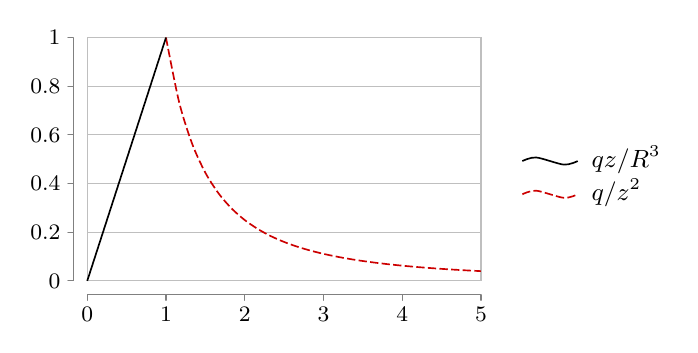
\begin{tikzpicture}
\datavisualization [scientific axes=clean,
                    y axis=grid,
                    visualize as smooth line/.list={inside,outside},
                    style sheet=strong colors,
                    style sheet=vary dashing,
                    inside={label in legend={text=$qz/R^3$}},
                    outside={label in legend={text=$q/z^2$}},
                    data/format=function
                    ]
data [set=inside] {
  var x : interval [0.0:1.0];
  func y = \value x;
}
data [set=outside] {
  var x : interval [1.0:5.0];
  func y = 1.0/(\value x*\value x);
};
\end{tikzpicture}

\section{DIVERGENCE AND CURL OF ELECTROSTATIC FIELDS}
\subsection{Field Lines, Flux and Gauss-s Law}

Equation \ref{eq:G01_electrostatic_field_continuous_vol} is the recipe for computing the electric \tit{field} of a charge distribution, then equation \ref{eq:G01_electrostatic_force} tells us what the \tit{force} on a charge $Q$ placed in this field will be. The integrals involved in computing $\vb{E}$ can be very difficult to calculate, even for relatively simple charge distributions. One then often exploits certain properties of the electric field by which the latter can be determined without an explicit calculation of the integral in \ref{eq:G01_electrostatic_field_continuous_vol}. 

Much can be understood about a vector field $\vb{E}$ by the values of its \tit{divergence} and \tit{curl}. There is indeed a general result of vector calculus -- Helmoltz's Theorem -- by which any vector field $\vb{A}$ that is sufficiently smooth and satisfying appropriate boundary conditions can be decomposed into the sum of a \tit{curl-free} ($\curl{\vb{A}}=\vb{0}$) field plus a \tit{divergence-free} ($\div{\vb{A}}=0$) field.     

$\vb{E}$ is a  \tit{curl-free} vector field and this is a consequence of 
\begin{itemize}
\item it being \tit{linearly} dependent on the source charges, so that a \tit{superposition principle} holds; 
\item it being directed \tit{radially} from any infinitesimal charge-carrying volume $d\tau$, so that integrating over a path that lies on a spherical surface centered on the source charge yields \tit{zero}; 
\item its \tit{magnitude} at any point $\vb{r}$ being a function of the distance of that point from any infinitesimal charge-carrying volume $d\tau$ located at $\vb{r}'$ ($\abs{\vb{E}(\vb{r})} = f(\abs{\vb{r} - \vb{r}'})$)\footnote{Note that the following demonstration does not require the field to decay by an inverse-square law as the electric field does.}. 
\end{itemize}

The reasoning to demonstrate that $\vb{E}$ is \tit{curl-free} goes as follows:
\begin{itemize}[-]
\item By Stokes theorem of vector calculus, given $\Gamma$ any closed curve and $\Sigma$ any closed surface bounded by  $\Gamma$, the \tit{line-integral} of $\vb{E}$ along $\Gamma$ (also called the \tit{circulation} of $\vb{E}$) equals the \tit{surface-integral} of $\curl{\vb{E}}$ (also called the \tit{flux of rotation}). 
\item Any closed path $\Gamma$ can be approximated to any precision degree by a curve made of an infinite sequence of steps where each step consists of an infinitesimal \tit{radial} displacement followed by a displacement along a spherical surface centered on the source charge $d\tau$ located at $\vb{r}'$. The latter type of displacement in each step \tbf{contributes nothing} to the line integral of $\vb{E}$, because the field is at right-angle with the path.
\item Given that only \tit{radial displacements} contribute to the line integral of $\vb{E}$ the latter must vanish on any closed path, since all outwardly directed displacements must be compensated by an equivalent amount of inwardly directed ones in order for the path to close.    
\item Due to the superposition principle, the vanishing of the \tit{circulation} thus holds for any field $\vb{E}$ and this in turn implies the vanishing of the \tit{flux of rotation}. The vanishing of the latter over the infinitely many surfaces bounded by an arbitrarily chosen curve $\Gamma$ clearly requires that $\curl{\vb{E}}=\vb{0}$.     
\end{itemize}
%\footnote{This is true also of fields generated by charges that are not static.}  % Griffiths - Electrodynamics / Electrostatics
%\include{Griffiths_02}	 % Griffiths - Electrodynamics / Potentials
%\include{Griffiths_03}	 % Griffiths - Electrodynamics / Electric Fields in Matter
%\include{Griffiths_04}	 % Griffiths - Electrodynamics / Magnetostatics
%\include{Griffiths_05}	 % Griffiths - Electrodynamics / Magnetic Fields in Matter
%\include{Griffiths_06}	 % Griffiths - Electrodynamics / Electrodynamics
%\include{Griffiths_07}	 % Griffiths - Electrodynamics / Conservation Laws
%\include{Griffiths_08}	 % Griffiths - Electrodynamics / Electromagnetic Waves
%\include{Griffiths_09}	 % Griffiths - Electrodynamics / Radiation
%\include{Griffiths_10}	 % Griffiths - Electrodynamics / Electrodynamics and Relativity
%\include{Griffiths_11}	 % Griffiths - Electrodynamics / Potentials and Fields
%\include{Griffiths_12}	 % Griffiths - Electrodynamics / Helmoltz Theorem

%\chapter{Jackson -- Maxwell Equations, Conservation Laws}
\label{ch:Jackson_06} 

\section{Maxwell Equations}

\begin{equation}
\begin{aligned}
\div{\vb{B}} &= 0\\
\curl{\vb{E}} + \frac{1}{c} \pdv{\vb{B}}{t} &= 0\\
\div{\vb{E}} &= 4 \pi \rho\\
\curl{\vb{B}} &= \frac{4 \pi}{c} \vb{J} + \frac{1}{c} \pdv{\vb{E}}{t}
\end{aligned}
\label{eq:maxwell}
\end{equation}


\section{Potentials}

$\vb{B}$ has a vanishing divergence, therefore a vector field $\vb{A}$ exists such that

\begin{equation}
\vb{B} = \curl{\vb{A}}
\label{eq:Adef}
\end{equation}

Substituting \ref{eq:Adef} in the second of Maxwell equations one gets

\begin{equation*}
\curl{\vb{E}} + \frac{1}{c} \pdv{\curl{\vb{A}}}{t} = 0
\end{equation*}

whence 

\begin{equation}
\curl{ \left( \vb{E} + \frac{1}{c} \pdv{\vb{A}}{t} \right)} = 0
\end{equation}

The expression enclosed in parentheses in the above equation implies that a scalar field $\phi$ exists such that 

\begin{equation}
\vb{E} + \frac{1}{c} \pdv{\vb{A}}{t} = - \grad{\phi}
\label{eq:phidef}
\end{equation}


Using the last equation in \ref{eq:maxwell} and a known theorem of vector calculus

\begin{align*}
\curl{\vb{B}} &= \curl{(\curl{\vb{A}})} \\
&= \grad{(\div{\vb{A}})} - \laplacian{\vb{A}} \\
&= \frac{4 \pi}{c} \vb{J} + \frac{1}{c} \pdv{\vb{E}}{t}
\end{align*}

while from \ref{eq:phidef}

\begin{align*}
\frac{1}{c} \pdv{\vb{E}}{t} = - \frac{1}{c} \pdv{\grad{\phi}}{t} - \frac{1}{c^2} \pdv[2]{\vb{A}}{t}  
\end{align*}

therefore

\begin{align*}
\grad{(\div{\vb{A}})} - \laplacian{\vb{A}} &= \frac{4 \pi}{c} \vb{J} + \frac{1}{c} \pdv{\vb{E}}{t} \\
&= \frac{4 \pi}{c} \vb{J} - \frac{1}{c} \pdv{\grad{\phi}}{t} - \frac{1}{c^2} \pdv[2]{\vb{A}}{t}  
\end{align*}

With the goal of arriving at two independent equations for $\phi$ and $\vb{A}$ we put the equation for $\vb{A}$ in the following form 

\begin{equation}
\begin{aligned}
\laplacian{\vb{A}} - \frac{1}{c^2} \pdv[2]{\vb{A}}{t} &= - \frac{4 \pi}{c} \vb{J} \\
&+ \grad{\left( \div{\vb{A}} + \frac{1}{c} \pdv{\phi}{t} \right)}
\label{eq:uglyA}
\end{aligned}
\end{equation}

Turning to the scalar potential $\phi$ and combining the third equation in \ref{eq:maxwell} with \ref{eq:phidef} we obtain 

\begin{equation}
\begin{aligned}
\div{\vb{E}} &=   4 \pi \rho \\
&= - \laplacian{\phi} - \frac{1}{c} \pdv{\div{\vb{A}}}{t}
\label{eq:uglyPhi}
\end{aligned}
\end{equation}

\section{Gauge transformations}
Equations \ref{eq:uglyA} and \ref{eq:uglyPhi} are interdependent: one cannot be solved without the other having been solved. They stem from equations \ref{eq:Adef} and \ref{eq:phidef}, where potentials were introduced (respectively $\vb{A}$ and $\phi$) to yield fields $\vb{B}$ and $\vb{E}$ that by construction satisfy two of the four Maxwell equations \ref{eq:maxwell} (the homogeneous ones). 
However, the equations \ref{eq:Adef} and \ref{eq:phidef} do not uniquely determine the potentials. Indeed, if 
$\vb{A}$ and $\phi$ satisfy the equations, the same is true of the potentials $\vb{A}'$ and $\phi'$ obtained with the following transformation

\begin{equation}
\begin{aligned}
\vb{A}  &\longrightarrow \: \vb{A}' = \vb{A} + \grad{\lambda(\vb{r}, t)} \\   
\phi    &\longrightarrow \: \phi' = \phi - \frac{1}{c} \pdv{\lambda(\vb{r}, t)}{t}   
\label{eq:gaugexform}
\end{aligned}
\end{equation}

where $\lambda(\vb{r}, t)$ is any scalar function of position and time.

\subsection{Lorenz gauge}

Imposing the following constraint (\textit{Lorenz gauge}) on the potentials $\phi$ and $\vb{A}$

\begin{equation}
\div{\vb{A}} + \frac{1}{c} \pdv{\phi}{t} = 0
\label{eq:lorenzgauge} % Yes this is from Lorenz, not from the other (Lorentz)
\end{equation}

amounts to apply the transformation \ref{eq:gaugexform} with $\lambda(\vb{r}, t)$ satisfying the following equation: 

\begin{align*}
\laplacian{\lambda} - \frac{1}{c^2} \pdv[2]{\lambda}{t} = \div{\vb{A}} + \frac{1}{c} \pdv{\phi}{t}
\end{align*}


As a result, one obtains two independent \textit{wave equations} governing the dynamics of $\phi$ and $\vb{A}$, where the \textit{source fields} $\rho$ and $\vb{J}$ appear in the respective inhomogeneous terms: 


\begin{equation}
\laplacian{\phi} - \frac{1}{c^2} \pdv[2]{\phi}{t} = - 4 \pi \rho
\label{eq:PhiWave}
\end{equation}

\begin{equation}
\laplacian{\vb{A}} - \frac{1}{c^2} \pdv[2]{\vb{A}}{t} = - \frac{4 \pi}{c} \vb{J} 
\label{eq:AWave}
\end{equation}


\subsection{Coulomb gauge}

 

 




    % J.D. Jackson -- Classical Electrodynamics, 2nd Edition
%\include{Jackson_07}    % J.D. Jackson -- Classical Electrodynamics, 2nd Edition

%\include{Jackson_11}    % J.D. Jackson -- Classical Electrodynamics, 3rd Edition
%\include{Jackson_12}    % J.D. Jackson -- Classical Electrodynamics, 3rd Edition

%\include{Franklin_02}   % J. Franklin -- Advanced Mechanics and General Relativity
%\include{Franklin_03}   % J. Franklin -- Advanced Mechanics and General Relativity
%\include{Franklin_04}   % J. Franklin -- Advanced Mechanics and General Relativity
%\include{Franklin_05}   % J. Franklin -- Advanced Mechanics and General Relativity
%\include{Franklin_06}   % J. Franklin -- Advanced Mechanics and General Relativity

%\include{Landau_01}	 % L.D. Landau, E.M. Lifshitz -- Teoria dei Campi
%\include{Landau_02}	 % L.D. Landau, E.M. Lifshitz -- Teoria dei Campi

%\include{Jackson_13}	 % J.D. Jackson -- Classical Electrodynamics, 3rd Edition
%\include{Jackson_14}	 % J.D. Jackson -- Classical Electrodynamics, 3rd Edition
%\include{Jackson_15}	 % J.D. Jackson -- Classical Electrodynamics, 3rd Edition
%\include{Jackson_16}	 % J.D. Jackson -- Classical Electrodynamics, 3rd Edition

%\include{MTWheeler_02}	 % C.W. Misner, K.S. Thorne, J.A. Wheeler -- Gravitation
%\include{MTWheeler_03}	 % C.W. Misner, K.S. Thorne, J.A. Wheeler -- Gravitation
%\include{MTWheeler_04}	 % C.W. Misner, K.S. Thorne, J.A. Wheeler -- Gravitation

%\include{Landau_03}	 % L.D. Landau, E.M. Lifshitz -- Teoria dei Campi
%\include{Landau_04}	 % L.D. Landau, E.M. Lifshitz -- Teoria dei Campi
%\include{Landau_05}	 % L.D. Landau, E.M. Lifshitz -- Teoria dei Campi
%\include{Landau_06}	 % L.D. Landau, E.M. Lifshitz -- Teoria dei Campi
%\include{Landau_07}	 % L.D. Landau, E.M. Lifshitz -- Teoria dei Campi
%\include{Landau_08}	 % L.D. Landau, E.M. Lifshitz -- Teoria dei Campi
%\include{Landau_09}	 % L.D. Landau, E.M. Lifshitz -- Teoria dei Campi

%\appendixpage
%\appendix
\chapter{Tensors}
\label{ch:Tensors} 

\section{Vector Algebra}
For the sake of fixing notation, let $\{\vu{i}, \vu{j}, \vu{k}\}$ be an \textit{orthonormal} basis of unit vectors in three-dimensional space, and the following a list of all possible scalar products of basis vectors. 
  
\begin{equation}
\begin{aligned} 
\vu{i}\vdot \vu{i} &= \vu{j} \vdot \vu{j} = \vu{k} \vdot \vu{k} = 1 \\ 
\vu{i} \vdot \vu{j} &= \vu{j} \vdot \vu{k} = \vu{k} \vdot \vu{i} = 0 
\label{eq:basis_dot_products}
\end{aligned}
\end{equation}

For a \textit{right-handed} basis, the following is a list of all possible \textit{vector} products of basis vectors.
  
\begin{equation}
\begin{aligned} 
\vu{i} \cross \vu{i} &= \vu{j} \cross \vu{j} = \vu{k} \cross \vu{k} = 0 \\ 
\vu{i} \cross \vu{j} &= \vu{k} = - \vu{j} \cross \vu{i}\\
\vu{j} \cross \vu{k} &= \vu{i} = - \vu{k} \cross \vu{j}\\
\vu{k} \cross \vu{i} &= \vu{j} = - \vu{i} \cross \vu{k}
\label{eq:basis_vector_products}
\end{aligned}
\end{equation}





\backmatter%%%%%%%%%%%%%%%%%%%%%%%%%%%%%%%%%%%%%%%%%%%%%%%%%%%%%%%
%%%%%%%%%%%%%%%%%%%%%%%%% referenc.tex %%%%%%%%%%%%%%%%%%%%%%%%%%%%%%
% sample references
% 
% Use this file as a template for your own input.
%
%%%%%%%%%%%%%%%%%%%%%%%% Springer-Verlag %%%%%%%%%%%%%%%%%%%%%%%%%%

%
% BibTeX users please use
% \bibliographystyle{}
% \bibliography{}
%
% Non-BibTeX users please use
\begin{thebibliography}{99.}
%
% and use \bibitem to create references.
%
% Use the following syntax and markup for your references
%
% Monograph
\bibitem{Griffiths_4th} D.J. Griffiths (2017)
Introduction to Electrodynamics. Cambridge University Press, Cambridge

% Monograph
\bibitem{Felsager_1981} B. Felsager (1981)
Geometry, Particles and Fields. Odense University Press

% Monograph
\bibitem{BudakFomin_1973} B.M. Budak, S.V. Fomin (1973)
Multiple Integrals, Field Theory and Series. Mir Publishers, Moscow

% Monograph
\bibitem{Postnikov_II_1982} Mikhail Postnikov (1982)
Lectures in Geometry, Semester II. Linear Algebra and Differential Geometry. Mir Publishers, Moscow

\end{thebibliography}

\printindex

%%%%%%%%%%%%%%%%%%%%%%%%%%%%%%%%%%%%%%%%%%%%%%%%%%%%%%%%%%%%%%%%%%%%%%

\end{document}





